\documentclass[tikz,border=2pt]{standalone}
\usepackage{amsmath,amssymb}
\usetikzlibrary{arrows.meta,calc,fit,matrix,positioning}
\begin{document}
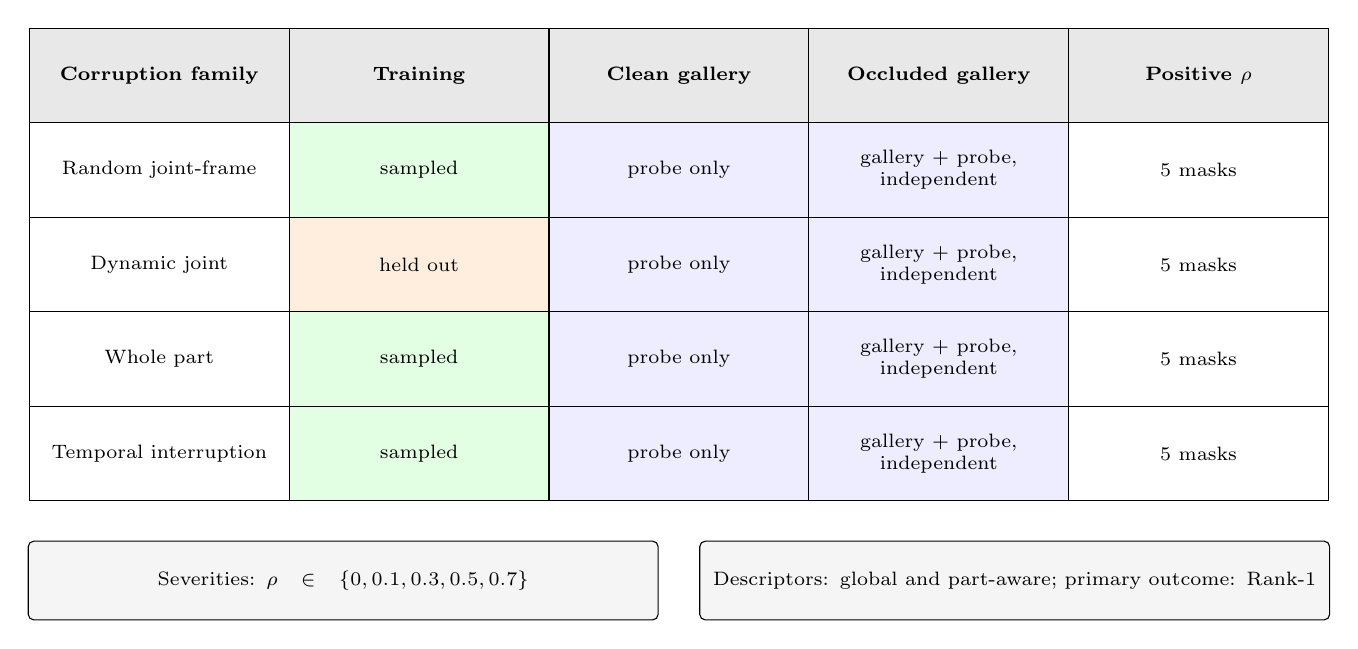
\begin{tikzpicture}[
    font=\scriptsize,
    cell/.style={draw, text width=30mm, minimum width=33mm,
        minimum height=12mm, inner sep=1.5mm, outer sep=0pt, align=center},
    family/.style={cell},
    train/.style={cell},
    clean/.style={cell},
    occ/.style={cell},
    reps/.style={cell},
    head/.style={fill=gray!18, font=\scriptsize\bfseries},
    yes/.style={fill=green!11},
    held/.style={fill=orange!13},
    protocol/.style={fill=blue!7}
]

\matrix (m) [matrix of nodes, nodes={anchor=center}, inner sep=0pt,
    row sep=-\pgflinewidth, column sep=-\pgflinewidth] {
    |[family,head]| Corruption family & |[train,head]| Training &
    |[clean,head]| Clean gallery & |[occ,head]| Occluded gallery &
    |[reps,head]| Positive $\rho$ \\
    |[family]| Random joint-frame & |[train,yes]| sampled &
    |[clean,protocol]| probe only & |[occ,protocol]| gallery + probe, independent &
    |[reps]| 5 masks \\
    |[family]| Dynamic joint & |[train,held]| held out &
    |[clean,protocol]| probe only & |[occ,protocol]| gallery + probe, independent &
    |[reps]| 5 masks \\
    |[family]| Whole part & |[train,yes]| sampled &
    |[clean,protocol]| probe only & |[occ,protocol]| gallery + probe, independent &
    |[reps]| 5 masks \\
    |[family]| Temporal interruption & |[train,yes]| sampled &
    |[clean,protocol]| probe only & |[occ,protocol]| gallery + probe, independent &
    |[reps]| 5 masks \\
};

\node[draw, rounded corners=2pt, fill=gray!8, align=center,
    text width=77mm, minimum width=80mm, minimum height=10mm,
    inner sep=1.5mm, outer sep=0pt, anchor=north west]
    (sev) at ([yshift=-5mm]m.south west)
    {Severities: $\rho\in\{0,0.1,0.3,0.5,0.7\}$};
\node[draw, rounded corners=2pt, fill=gray!8, align=center,
    text width=77mm, minimum width=80mm, minimum height=10mm,
    inner sep=1.5mm, outer sep=0pt, anchor=north east]
    (out) at ([yshift=-5mm]m.south east)
    {Descriptors: global and part-aware; primary outcome: Rank-1};

\end{tikzpicture}

\end{document}
